\section{Other works}
%----------------------------------------------------------------------------------------
\begin{frame}{Other works: SYK physics in disordered flatband systems}
    \begin{equation*}
        H = \eqnmarkbox[NavyBlue]{hoppings}{H_{t}}
        + \eqnmarkbox[OliveGreen]{disorder}{H_{D}}
        + \eqnmarkbox[WildStrawberry]{interaction}{H_{I}}
    \end{equation*}
    \annotate[yshift=0.5em]{above,left}{hoppings}{fermionic \& flatband}
    \annotate[yshift=0.5em]{above, right}{disorder}{disorder}
    \annotate[yshift=0.5em]{above, right}{interaction}{interaction}

    \vspace{-6.5mm}
    
    \begin{figure}
    \begin{minipage}{0.48\linewidth}
    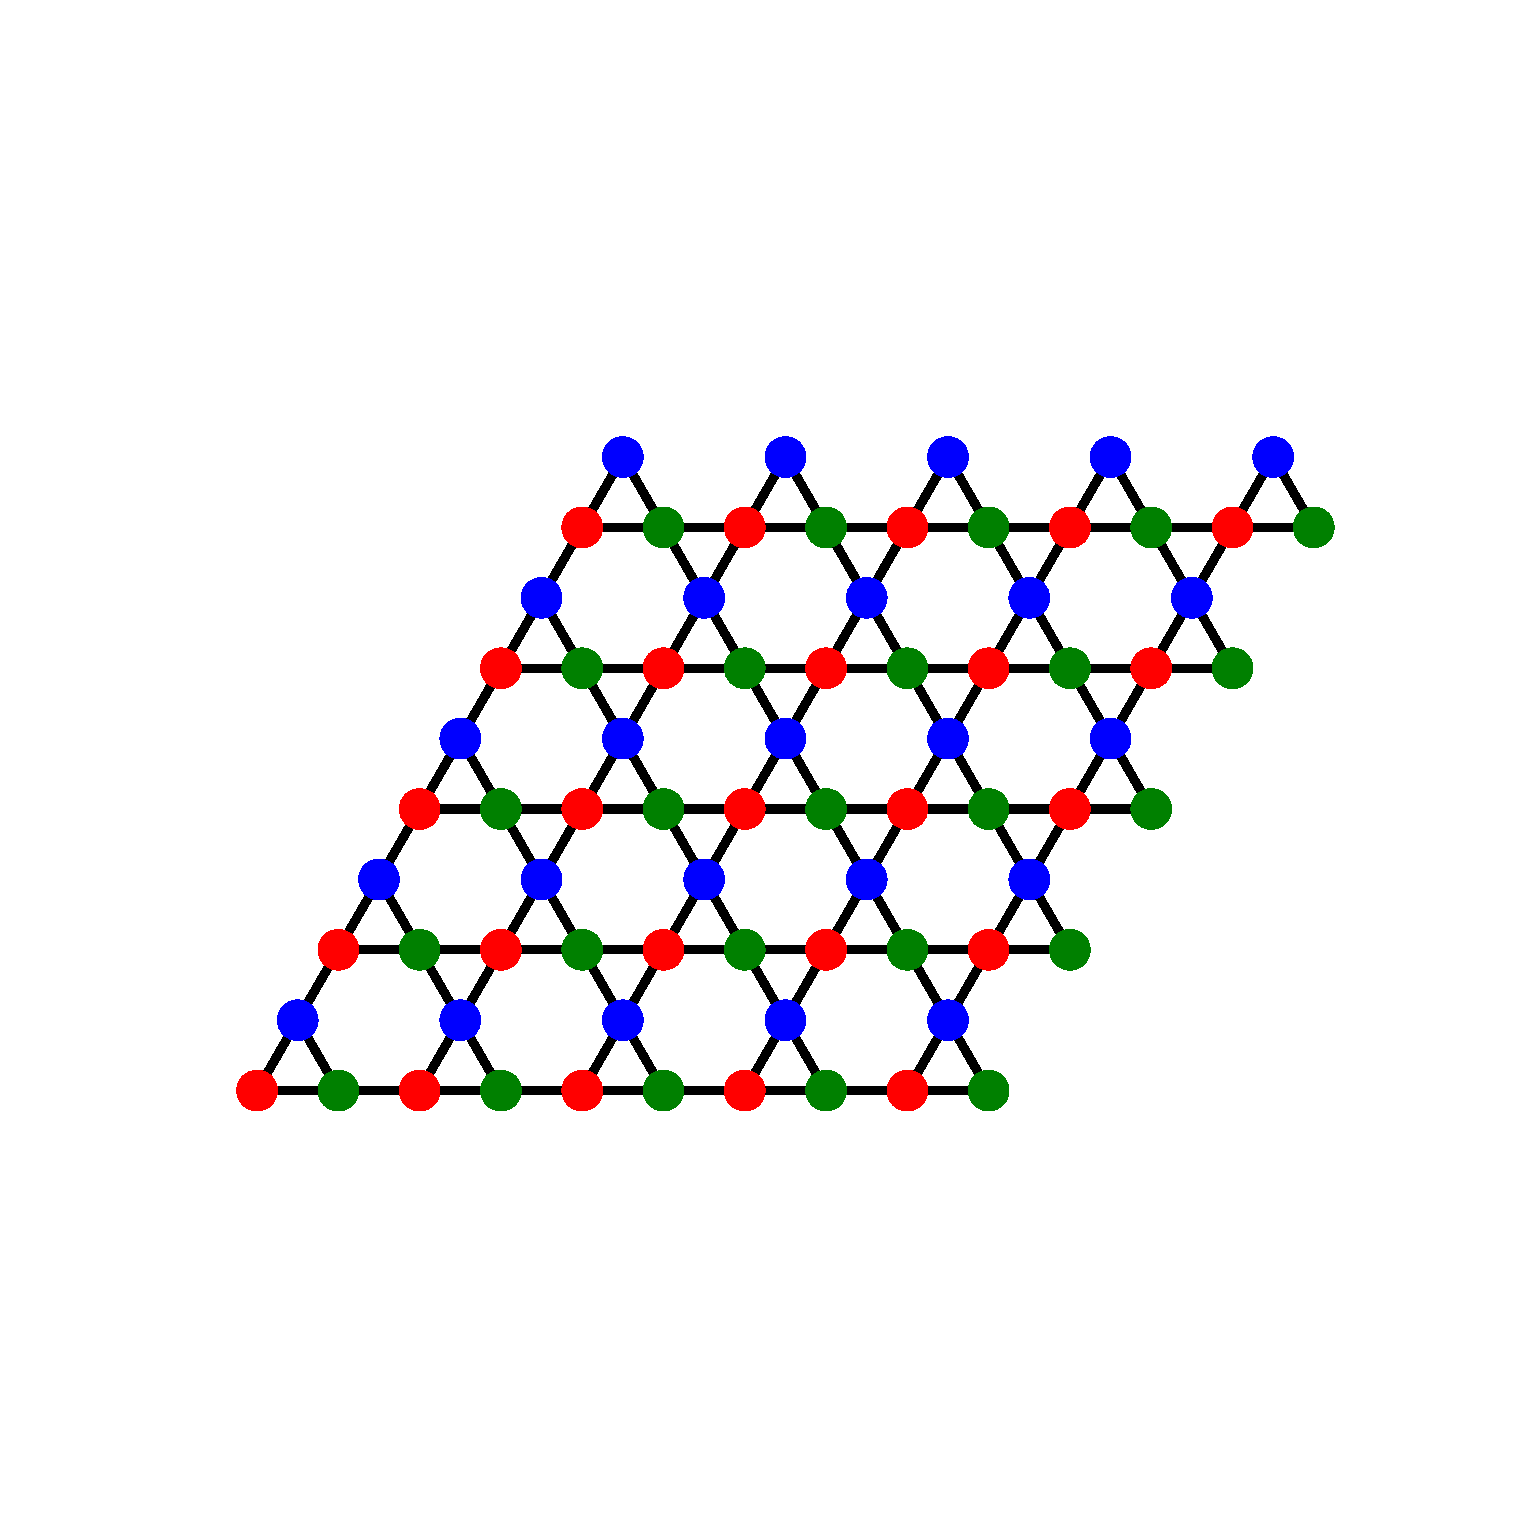
\includegraphics[width=0.49\linewidth,trim={20 20 20 20},clip]{figs/kagome/lattice.eps}
    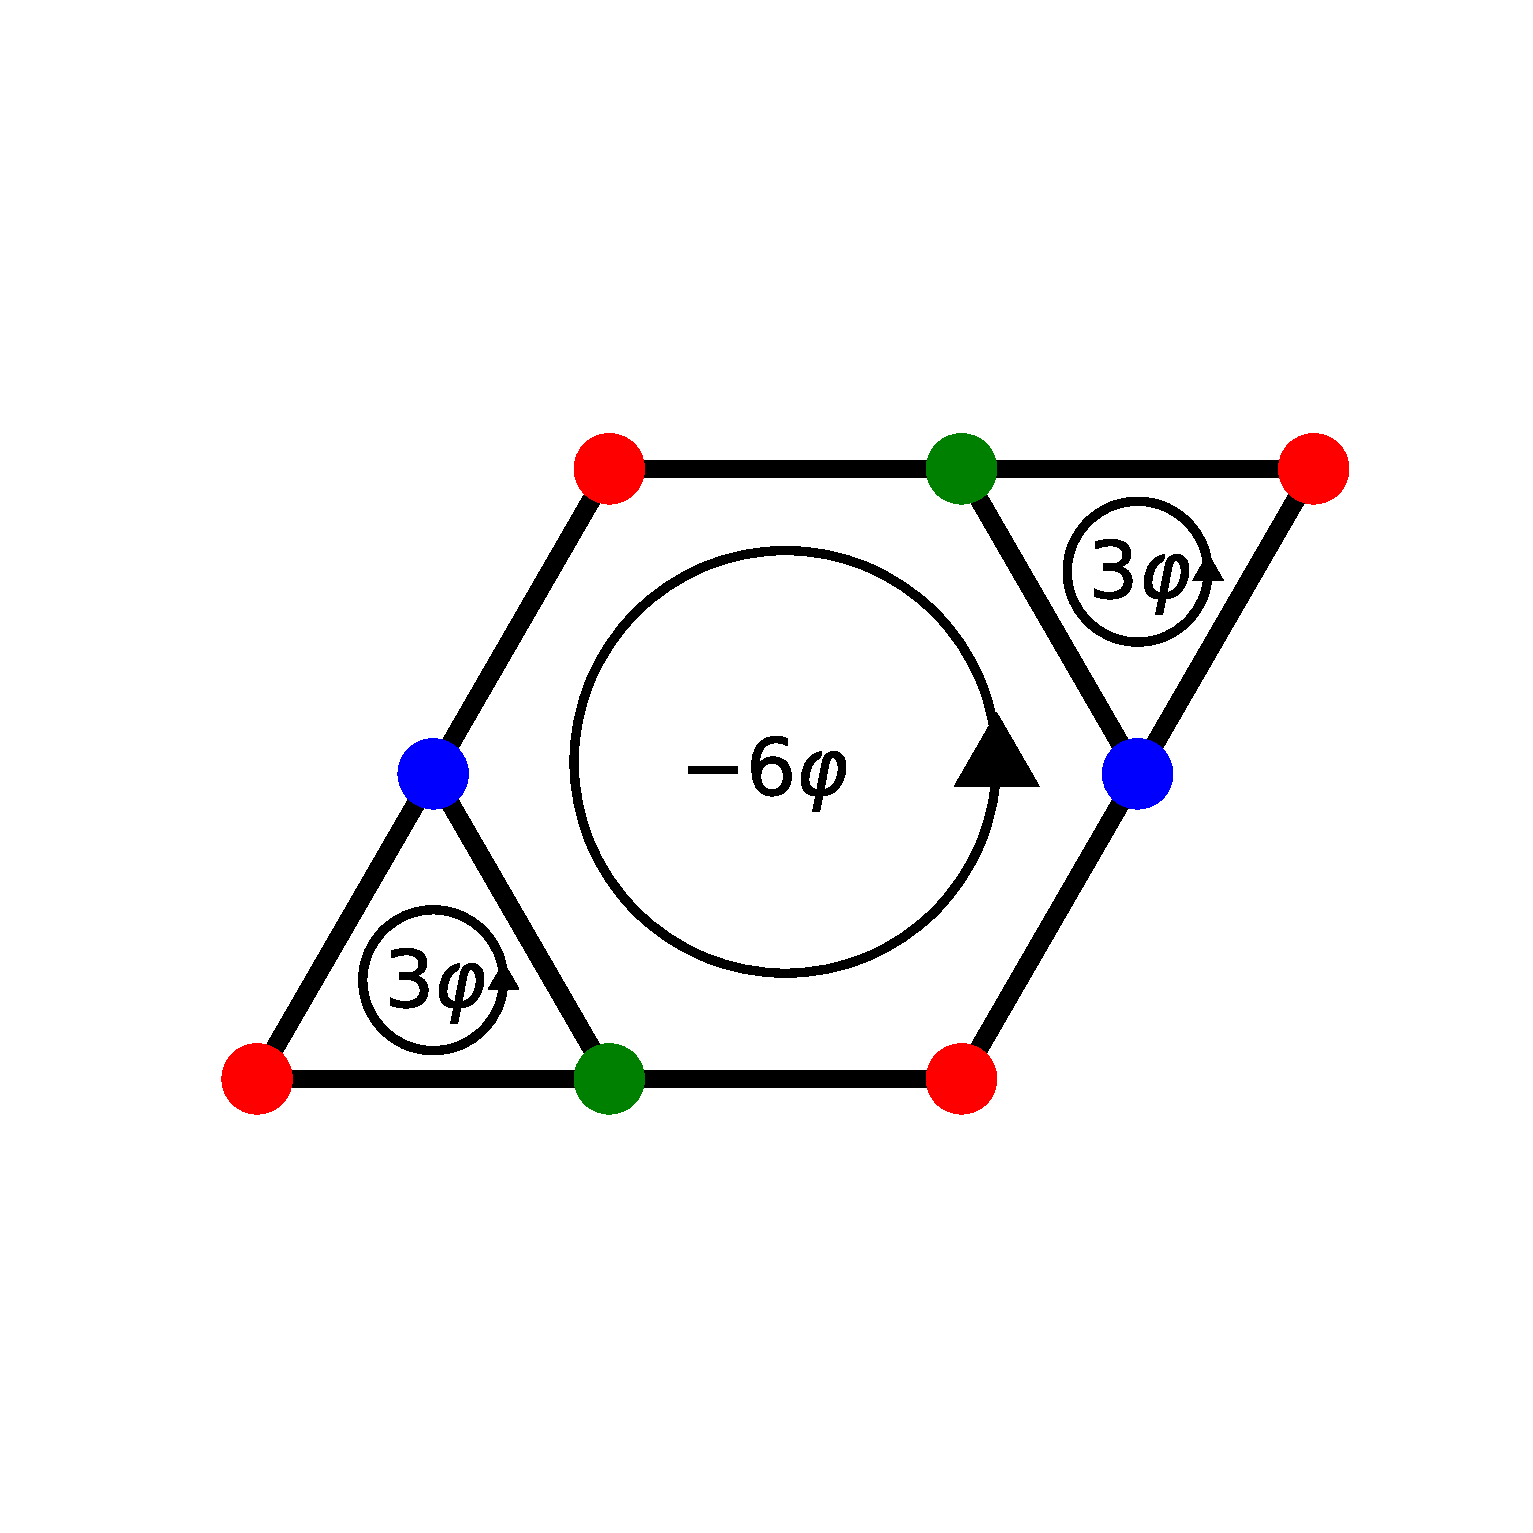
\includegraphics[width=0.49\linewidth]{figs/kagome/flux.eps}
    \begin{picture}(0,0)
    {\def\unitlength{}
    \put(0.338\linewidth,0.400\linewidth){\line(1,0){17pt}}
    \put(0.303\linewidth,0.334\linewidth){\line(1,0){17pt}}
    \put(0.303\linewidth,0.334\linewidth){\line(1,2){7pt}}
    \put(0.383\linewidth,0.334\linewidth){\line(1,2){7pt}}
    \put(0.41\linewidth,0.366\linewidth){\vector(1,0){55pt}}
    % \put(0.05\linewidth,0.1\linewidth){\small Localized states: $\ket{\mathbf{r}} = \frac{1}{\sqrt{6}} (\sum_{m}(-1)^{m}e^{2im\varphi}a_{\mathbf{r}_{m}}^{\dagger})\ket{0}$}
    }
    \end{picture}
    \end{minipage}
    \begin{minipage}{0.15\linewidth}
    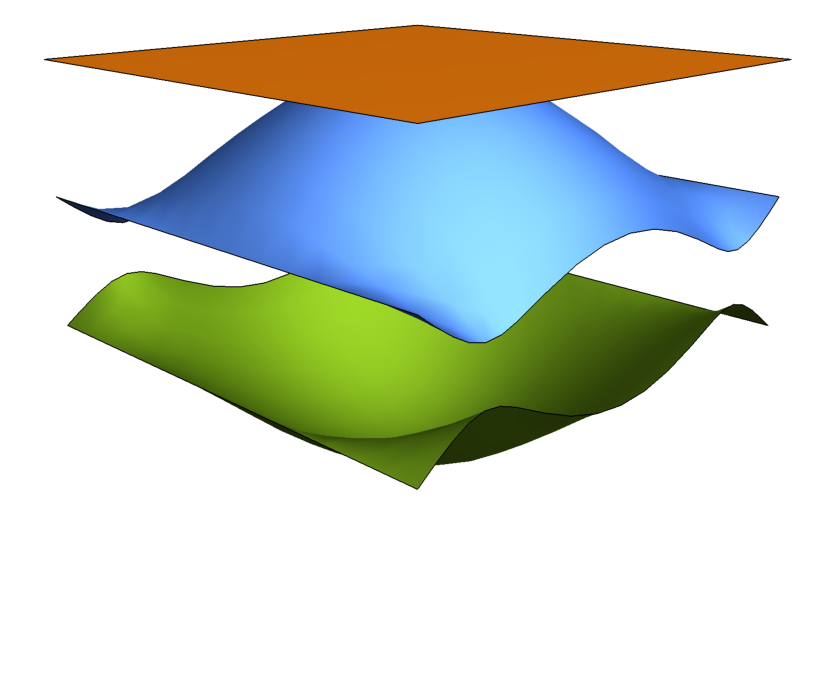
\includegraphics[trim={5 10 5 5},clip,width=\linewidth]{figs/kagome/Pi0.eps}
    \begin{picture}(0,0)
    {\def\unitlength{}
    \put(0.338\linewidth,0.1\linewidth){\text{$\varphi = 0$}}
    }
    \end{picture}
    \end{minipage}
    \begin{minipage}{0.15\linewidth}
    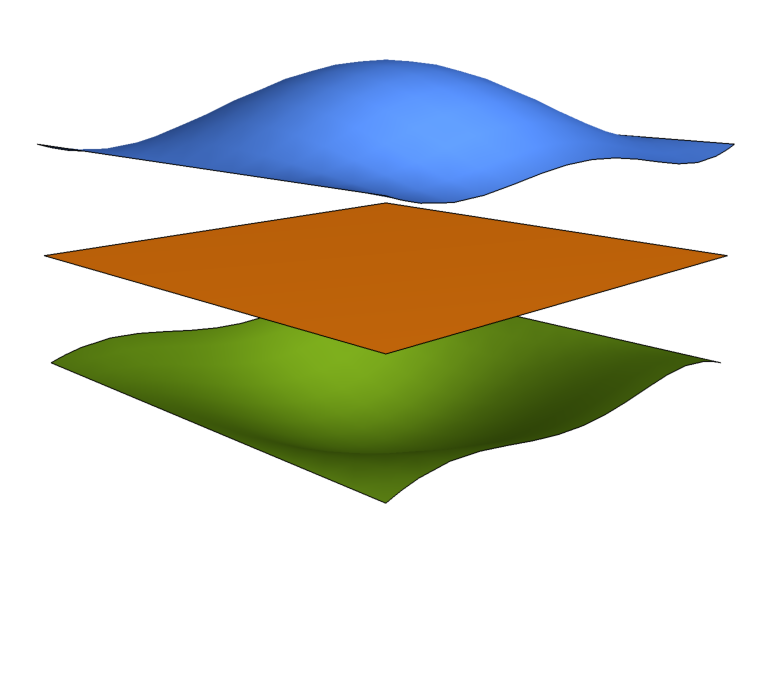
\includegraphics[trim={5 5 5 5},clip,width=\linewidth]{figs/kagome/Pi6.eps}
    \begin{picture}(0,0)
    {\def\unitlength{}
    \put(0.05\linewidth,0.1\linewidth){\text{$\varphi = \pi/6 \sim \pi/2$}}
    }
    \end{picture}
    \end{minipage}
    \begin{minipage}{0.15\linewidth}
    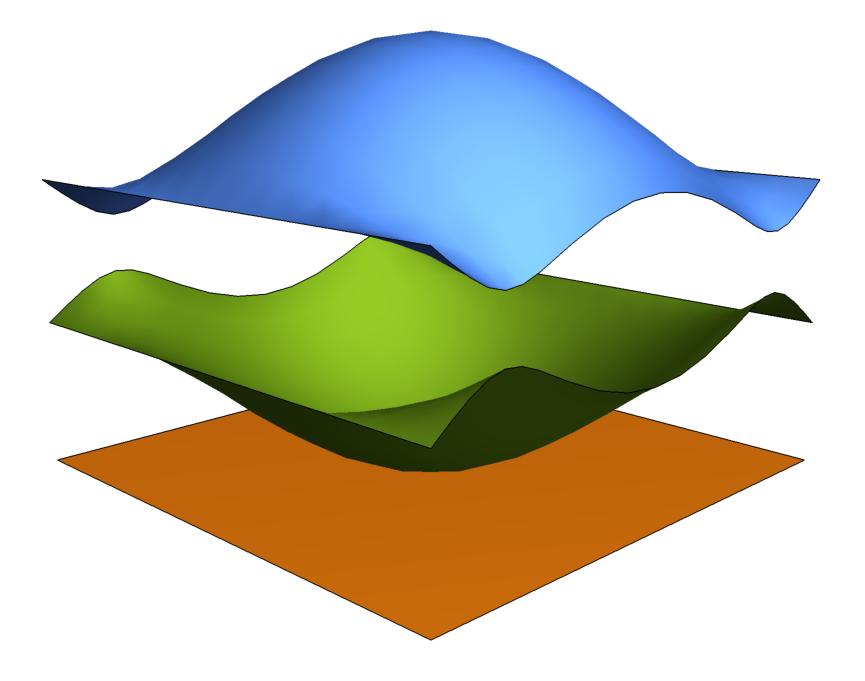
\includegraphics[trim={5 5 5 10},clip,width=\linewidth]{figs/kagome/Pi1.eps}
    \begin{picture}(0,0)
    {\def\unitlength{}
    \put(0.338\linewidth,0.1\linewidth){\text{$\varphi = \pi$}}
    }
    \end{picture}
    \end{minipage}
    \end{figure}

    \vspace{-12mm}

    \begin{figure}
    \begin{minipage}{0.24\textwidth}
    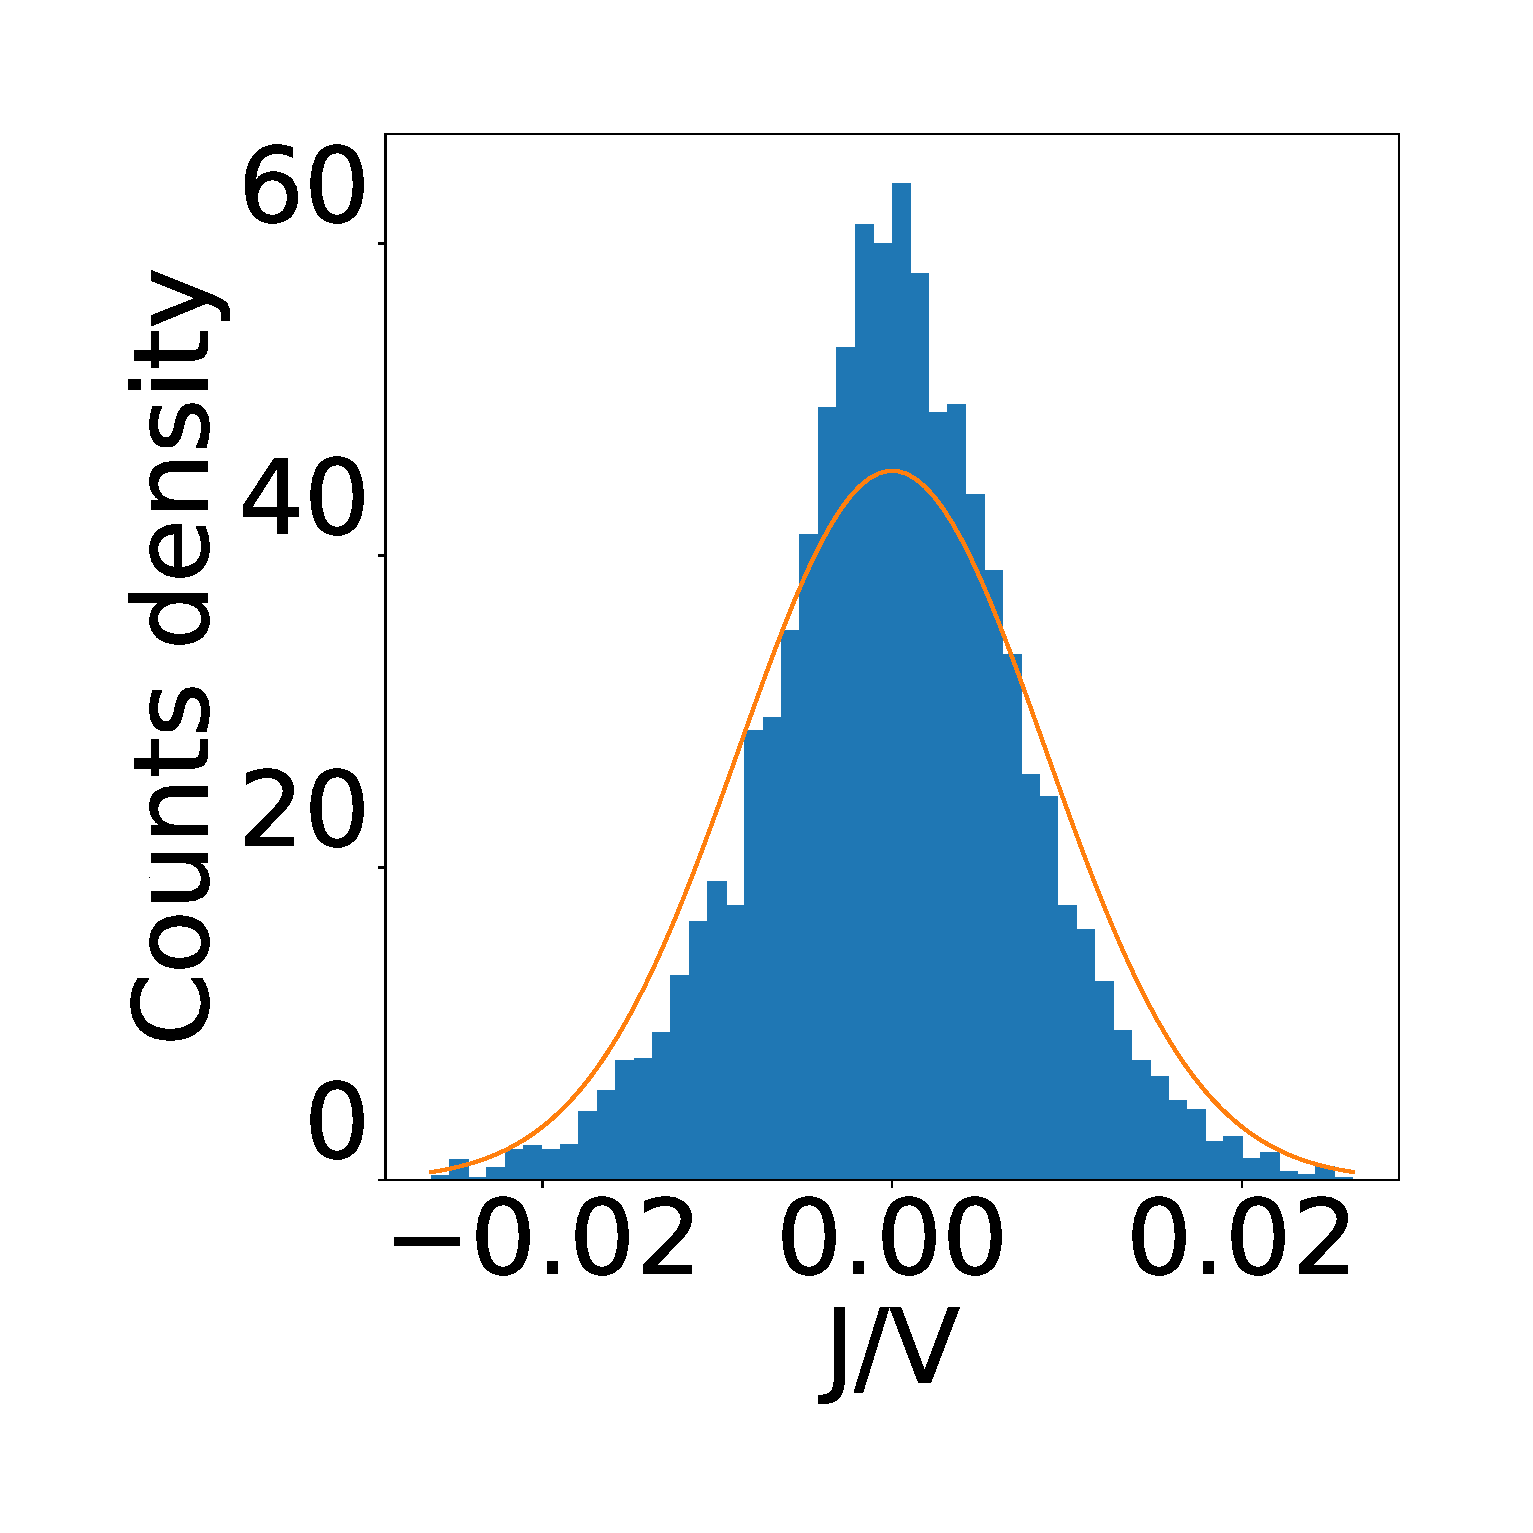
\includegraphics[width=\textwidth]{figs/kagome/1_J_15.eps}
    \begin{picture}(0,0)
    {\def\unitlength{}
    \put(0.69\linewidth,0.65\linewidth){\text{\tiny Gaussian}}
    \put(0.83\linewidth,0.63\linewidth){\vector(-1,-2){8pt}}
    }
    \end{picture}
    \end{minipage}
    \begin{minipage}{0.24\textwidth}
    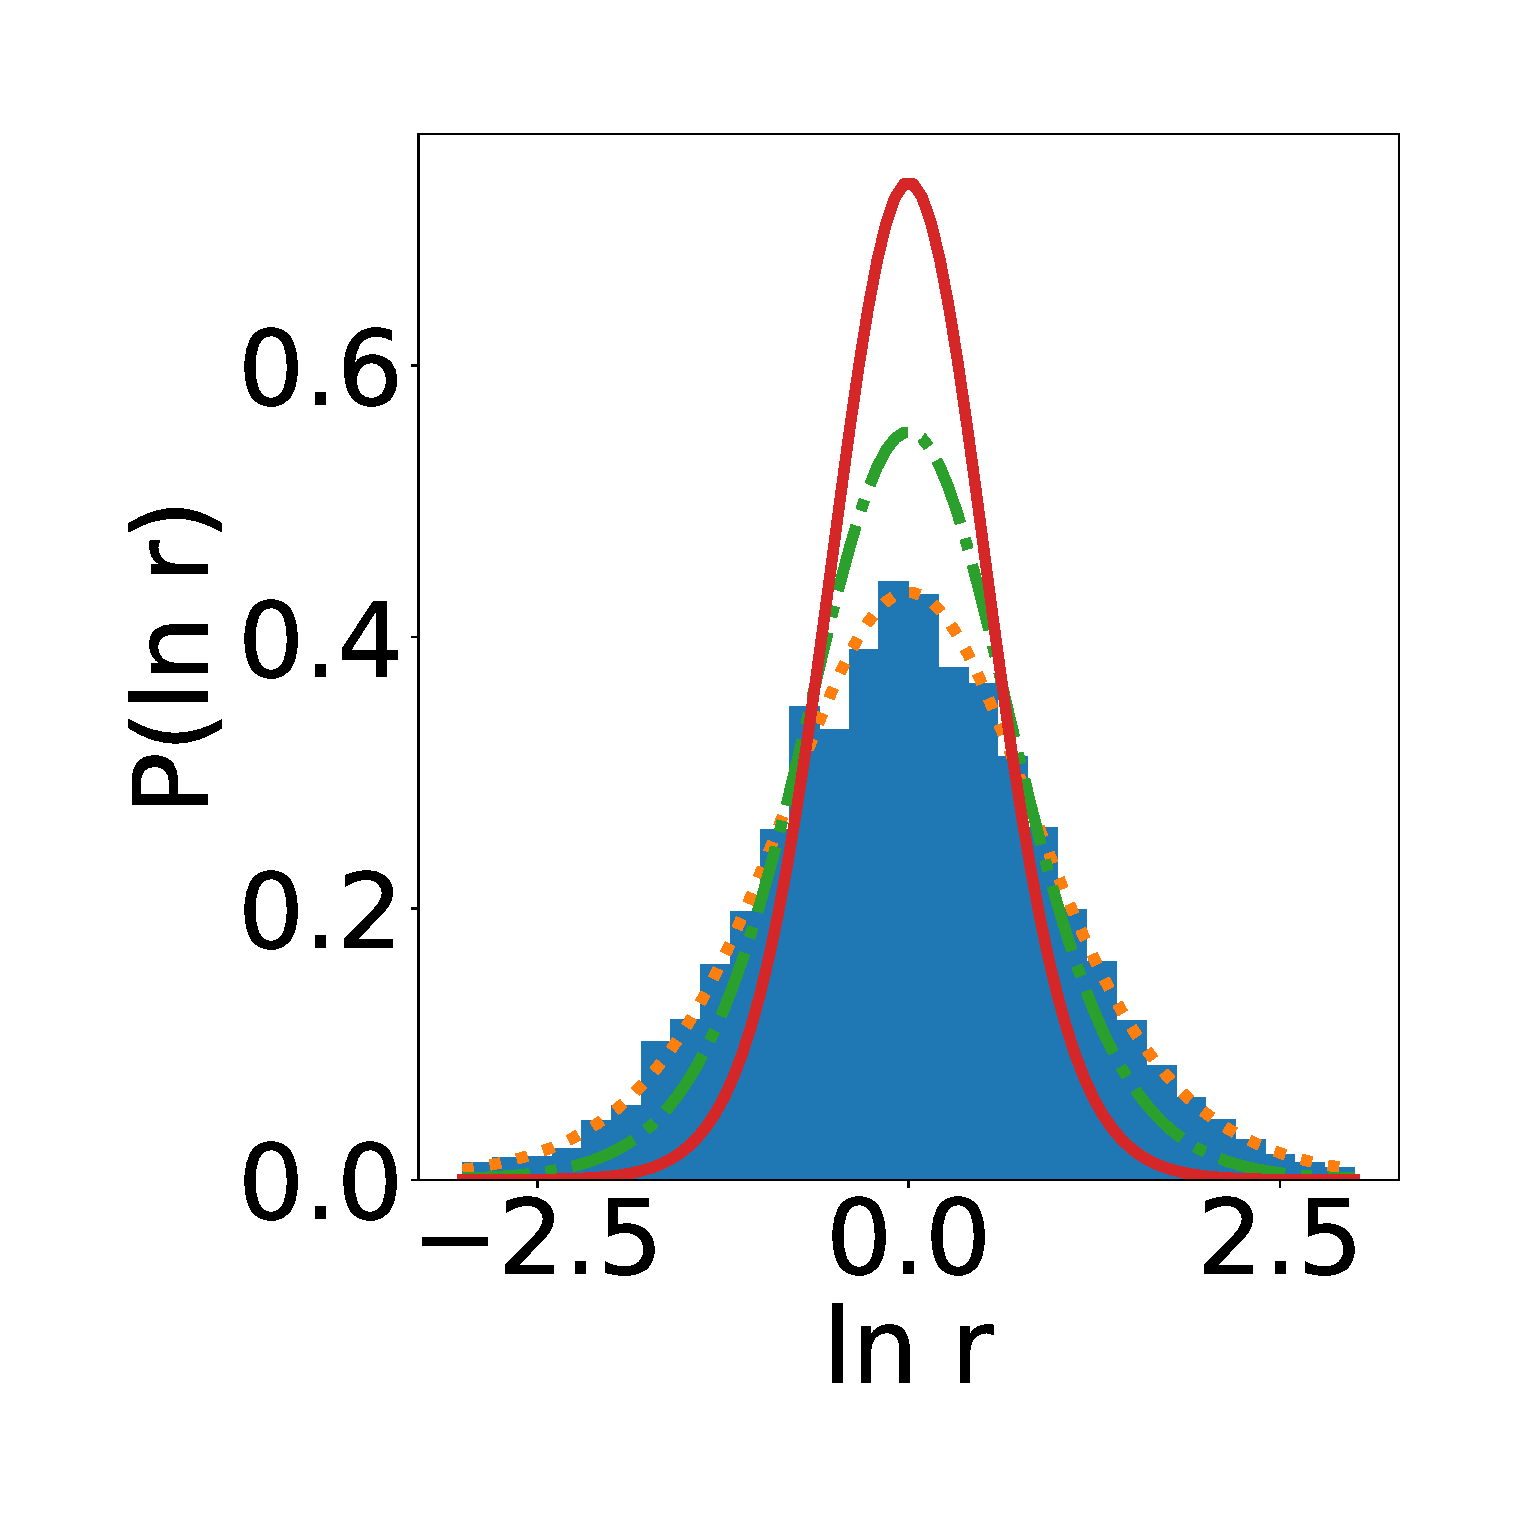
\includegraphics[width=\textwidth]{figs/kagome/1_r_15.eps}
    \begin{picture}(0,0)
    {\def\unitlength{}
    \put(0.8\linewidth,0.78\linewidth){\text{\tiny GSE}}
    \put(0.8\linewidth,0.8\linewidth){\vector(-1,0){16pt}}
    \put(0.8\linewidth,0.68\linewidth){\text{\tiny GUE}}
    \put(0.8\linewidth,0.7\linewidth){\vector(-1,0){15pt}}
    \put(0.8\linewidth,0.58\linewidth){\text{\tiny GOE}}
    \put(0.8\linewidth,0.6\linewidth){\vector(-1,0){14pt}}
    \put(0.35\linewidth,1.1\linewidth){\text{\tiny $r_{n}=\frac{E_{n+1}-E_{n}}{E_{n}-E_{n-1}}$}}
    }
    \end{picture}
    \end{minipage}
    \begin{minipage}{0.24\textwidth}
    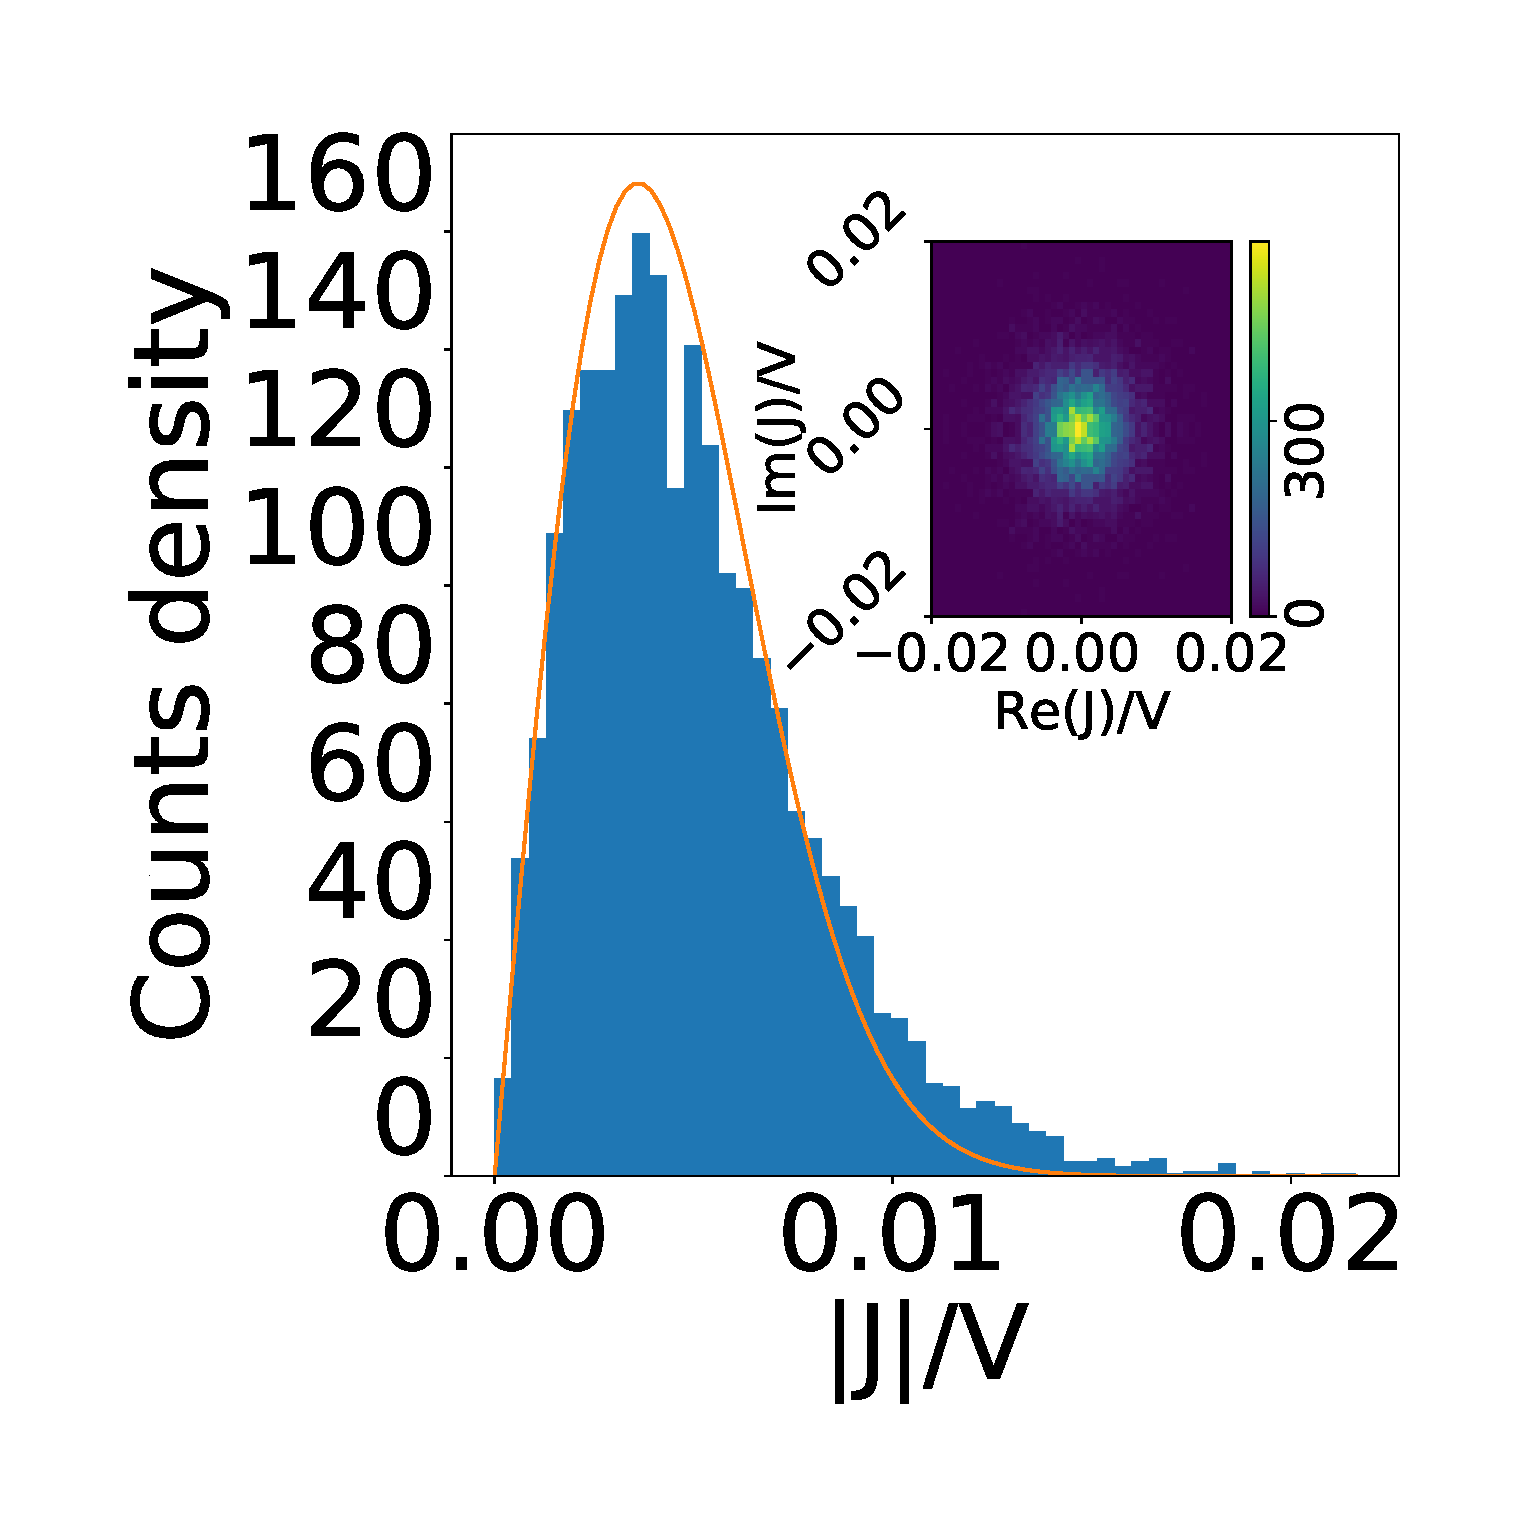
\includegraphics[width=\textwidth]{figs/kagome/T_J_15_insert.eps}
    \begin{picture}(0,0)
    {\def\unitlength{}
    \put(0.69\linewidth,0.58\linewidth){\text{\tiny Chi}}
    \put(0.68\linewidth,0.6\linewidth){\vector(-1,0){17pt}}
    }
    \end{picture}
    \end{minipage}
    \begin{minipage}{0.24\textwidth}
    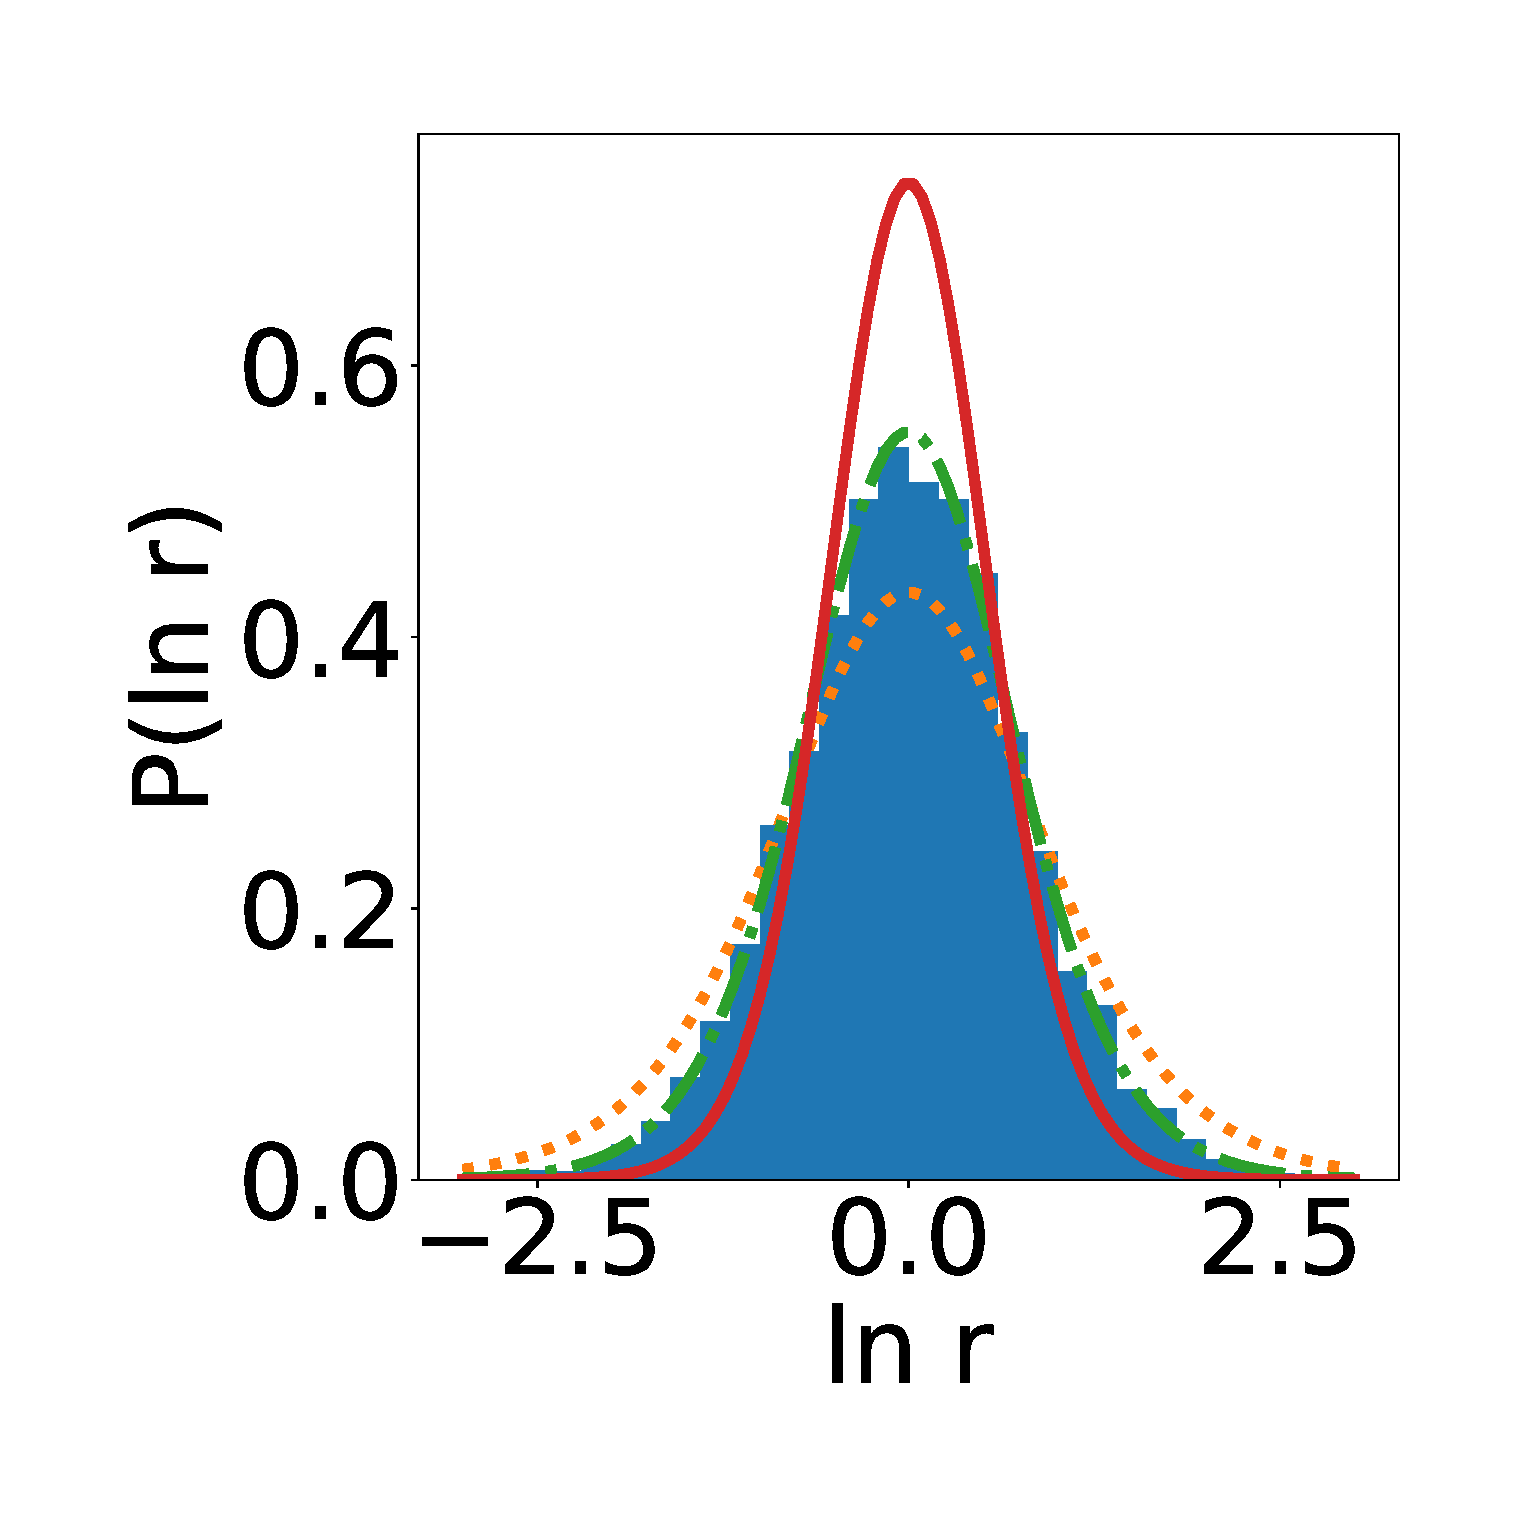
\includegraphics[width=\textwidth]{figs/kagome/T_r_15.eps}
    \begin{picture}(0,0)
    {\def\unitlength{}
    \put(0.8\linewidth,0.78\linewidth){\text{\tiny GSE}}
    \put(0.8\linewidth,0.8\linewidth){\vector(-1,0){16pt}}
    \put(0.8\linewidth,0.68\linewidth){\text{\tiny GUE}}
    \put(0.8\linewidth,0.7\linewidth){\vector(-1,0){15pt}}
    \put(0.8\linewidth,0.58\linewidth){\text{\tiny GOE}}
    \put(0.8\linewidth,0.6\linewidth){\vector(-1,0){14pt}}
    \put(0.35\linewidth,1.1\linewidth){\text{\tiny $r_{n}=\frac{E_{n+1}-E_{n}}{E_{n}-E_{n-1}}$}}
    }
    \end{picture}
    \end{minipage}
    \end{figure}
\end{frame}
%----------------------------------------------------------------------------------------
\begin{frame}{Other works: SYK physics in disordered flatband systems}
    \begin{figure}
        \centering
        \hfill
        \begin{minipage}{0.25\linewidth}
        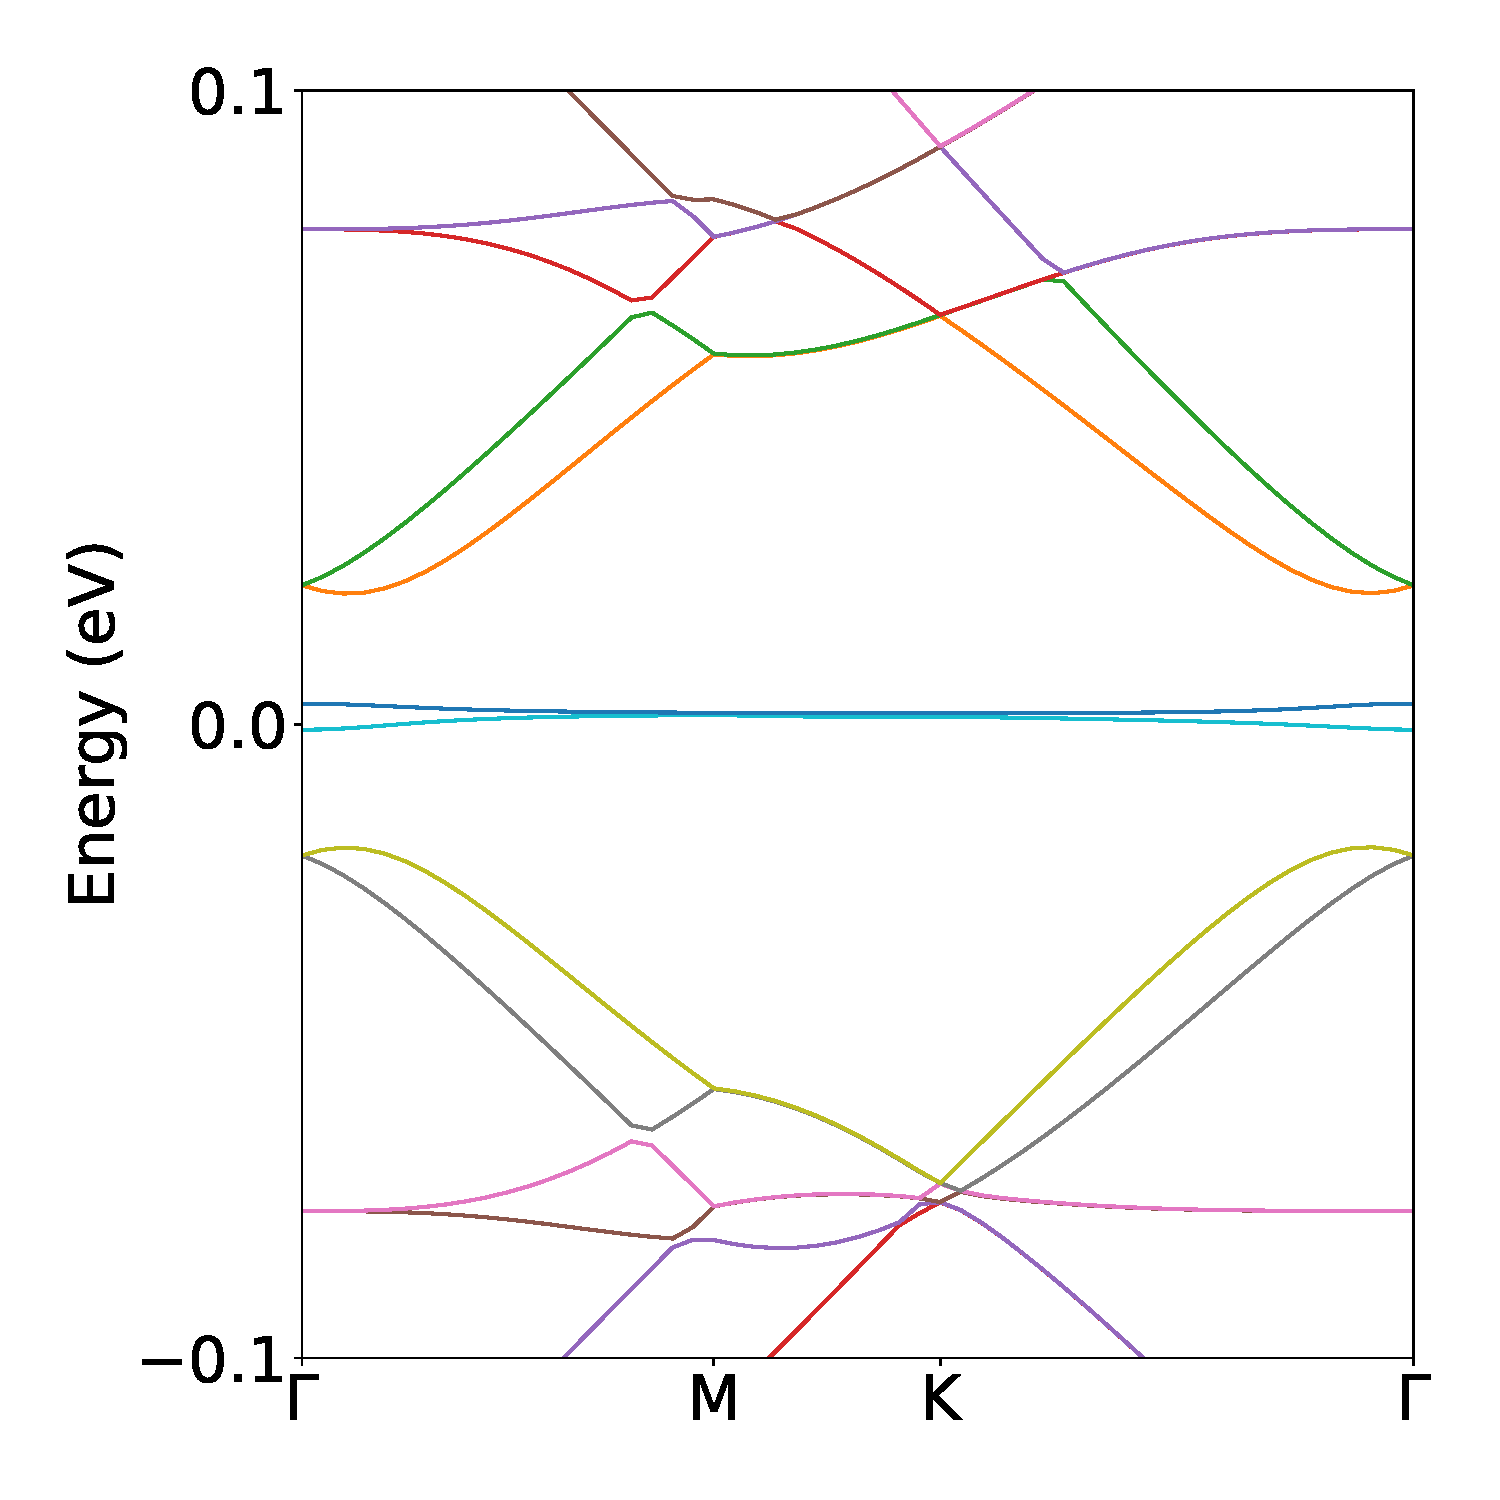
\includegraphics[width=\linewidth]{figs/SM/FlatBand.pdf}
        \end{minipage}
        \hfill
        \begin{minipage}{0.25\linewidth}
        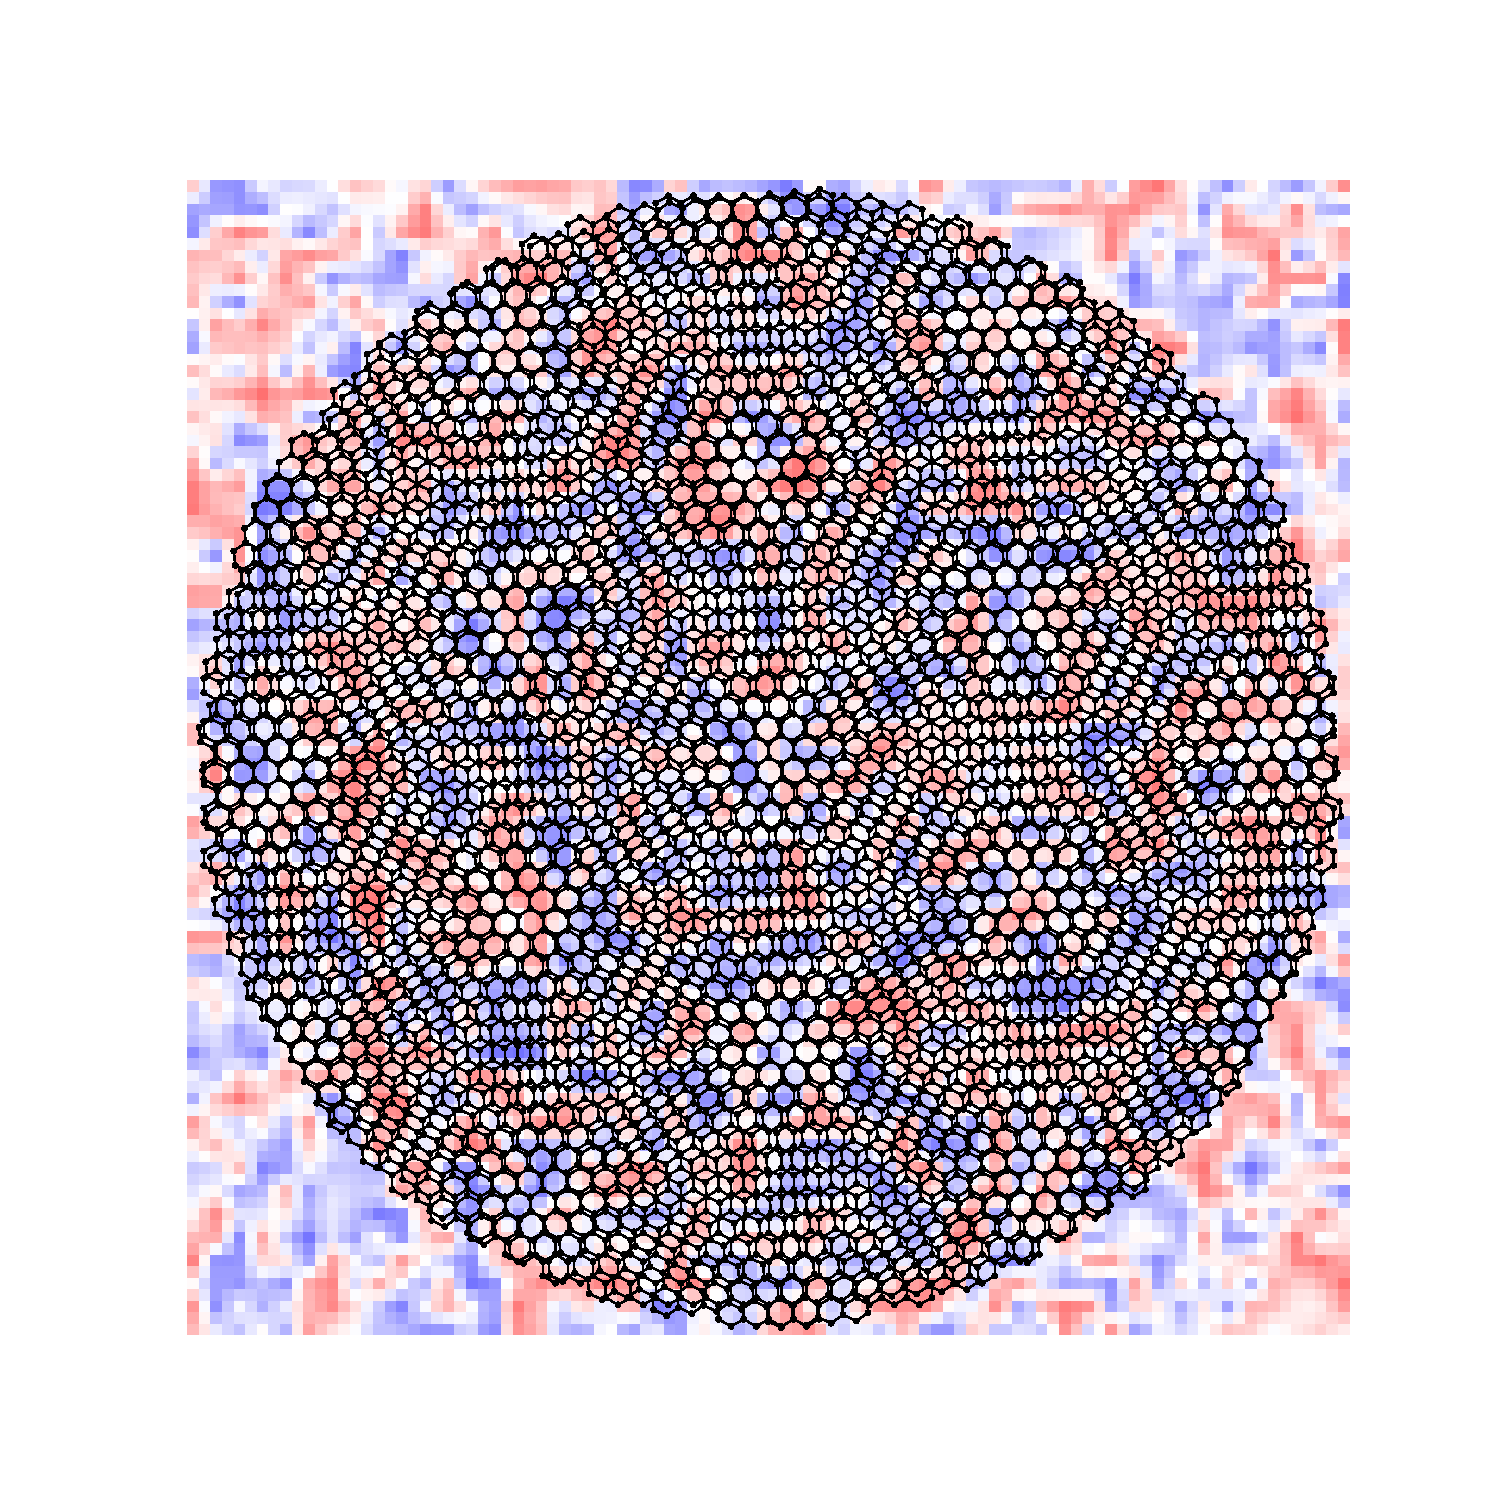
\includegraphics[width=\textwidth]{figs/SM/BLG.pdf}
        \end{minipage}
        \hfill
        \begin{minipage}{0.2\linewidth}
        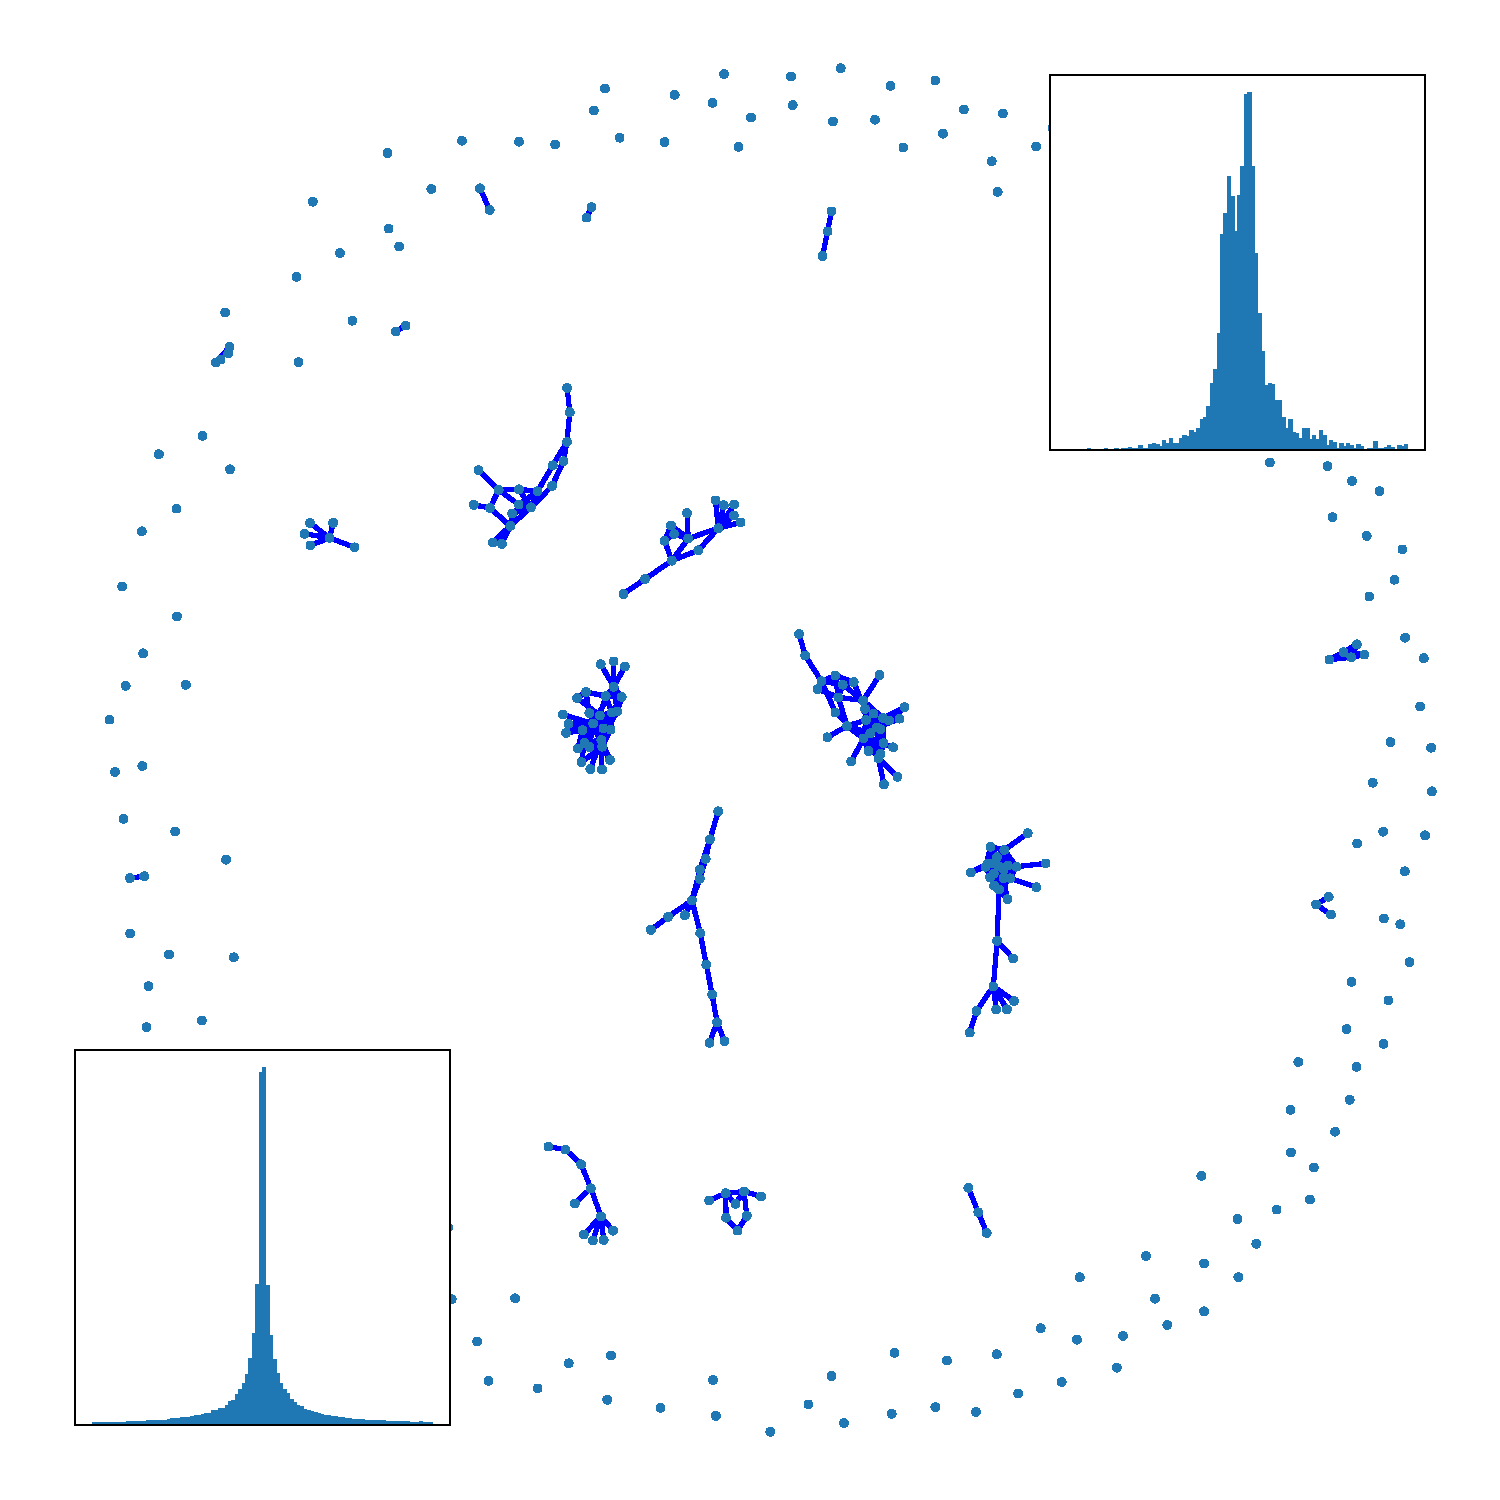
\includegraphics[width=\linewidth]{figs/SM/JTopo.pdf}
        \begin{picture}(0,0)
        {\def\unitlength{}
        % \put(-0.5\textwidth,\textwidth){$(b)$}
        \put(-0.05\linewidth,0.0\linewidth){$|J_{ijkl}|/\sigma_{\rm weak}$}
        \put(-0.04\linewidth,0.08\linewidth){$-1$}
        \put(0.28\linewidth,0.08\linewidth){$1$}
        \put(-0.05\linewidth,0.25\linewidth){$\rho$}
        \put(0.58\linewidth,0.65\linewidth){$|J_{ijkl}|/\sigma_{\rm strong}$}
        \put(0.61\linewidth,0.72\linewidth){$-3$}
        \put(0.93\linewidth,0.72\linewidth){$3$}
        \put(0.61\linewidth,0.9\linewidth){$\rho$}
        }
        \end{picture}
        \end{minipage}
        \hfill
        \begin{minipage}{0\linewidth}
        \end{minipage}
    \end{figure}
    \vspace{-5mm}
    \begin{figure}
        \centering
        \begin{minipage}{0.45\linewidth}
        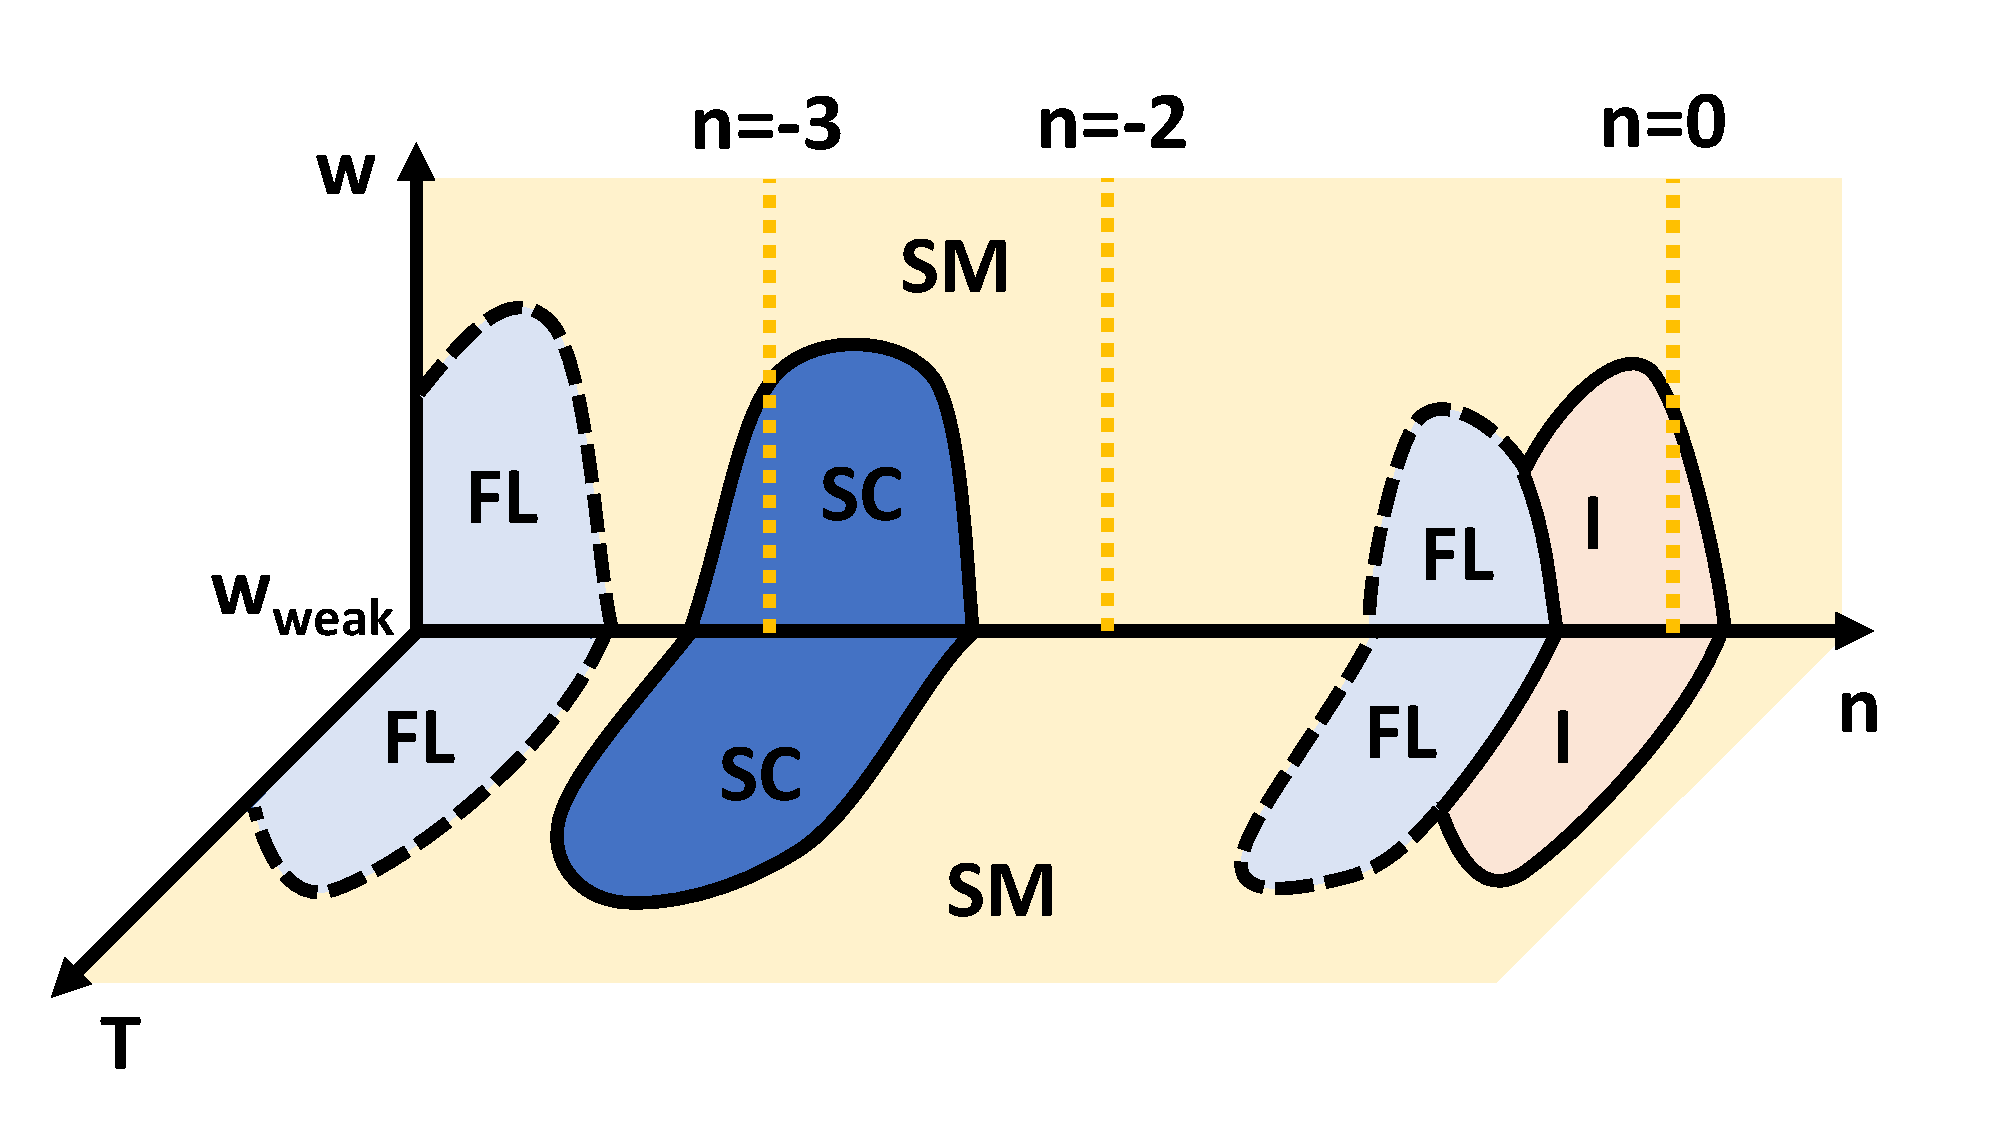
\includegraphics[width=\linewidth]{figs/SM/phase_diagram.pdf}
        \end{minipage}
    \end{figure}
\end{frame}
%----------------------------------------------------------------------------------------
\begin{frame}{Other works: chiral liquids}
\begin{columns}
\begin{column}{0.4\textwidth}
\begin{figure}
    \centering
    \begin{minipage}{1.0\linewidth}
    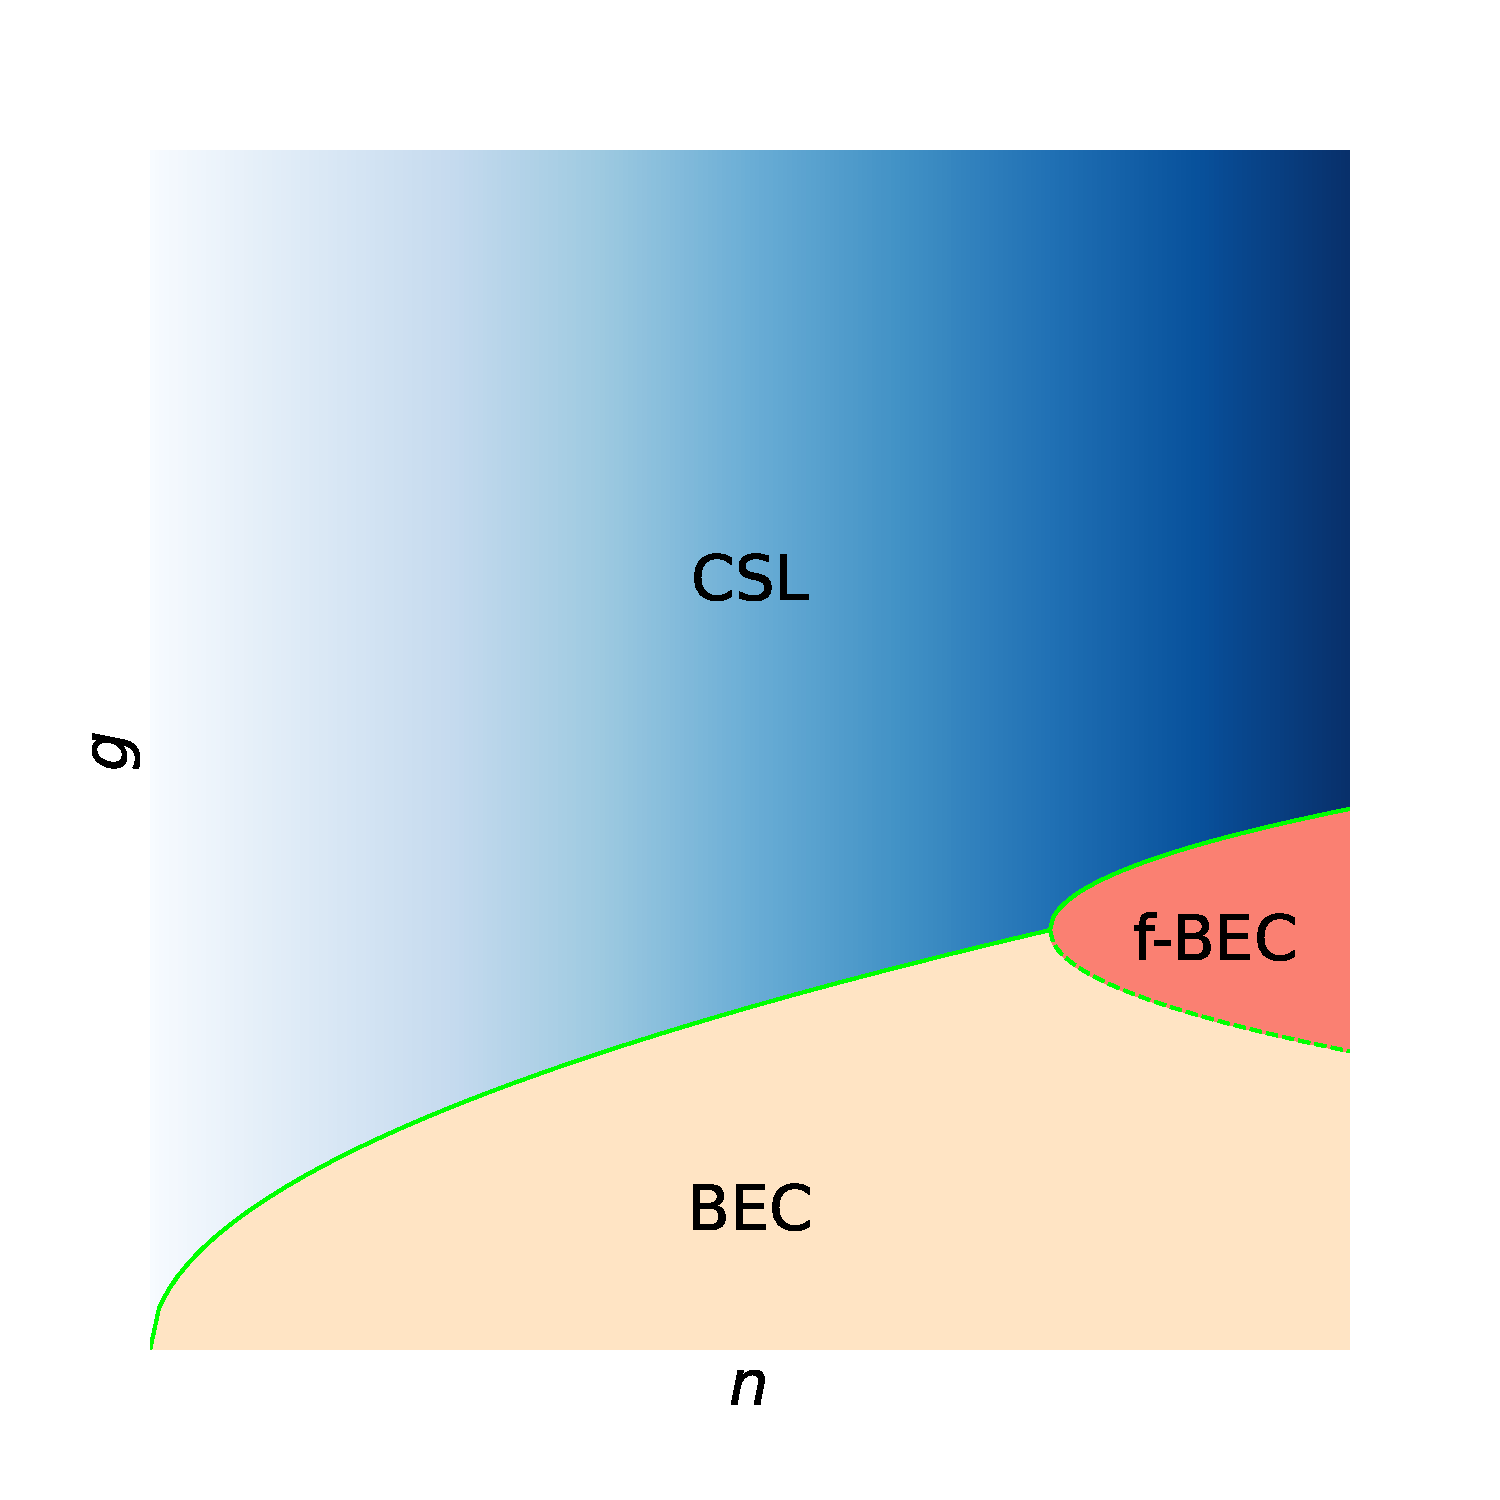
\includegraphics[width=\linewidth]{figs/CSL/PD.pdf}
    \begin{picture}(0,0)
    {\def\unitlength{}
    \put(0.44\textwidth,0.38\textwidth){\tiny $U(1)$ symmetry}
    \put(0.49\textwidth,0.35\textwidth){\tiny breaking}
    \put(0.61\textwidth,0.4\textwidth){\vector(2,1){0.12\textwidth}}
    \put(0.58\textwidth,0.35\textwidth){\vector(-2,-1){0.1\textwidth}}
    % \put(0.42\textwidth,0.68\textwidth){$E \sim n^{3.0}$}
    % \put(0.68\textwidth,0.82\textwidth){$E \sim n^{4/3}$}
    % \put(0.63\textwidth,0.3\textwidth){$E \sim gn$}
    \multiput(0.427\textwidth,0.19\textwidth)(0\textwidth,0.04\textwidth){20}{\line(0,1){0.02\textwidth}}
    \multiput(0.7\textwidth,0.19\textwidth)(0\textwidth,0.04\textwidth){7}{\line(0,1){0.02\textwidth}}
    \put(0.41\textwidth,0.1\textwidth){$n^*_1$}
    \put(0.62\textwidth,0.1\textwidth){$n^*_2 \sim 1.64n^*_1$}
    \put(0.25\textwidth,0.79\textwidth){\tiny Non-uniformity increasing}

    \multiput(0.11\textwidth,0.465\textwidth)(0.04\textwidth,0\textwidth){15}{\line(1,0){0.02\textwidth}}
    \put(0\textwidth,0.39\textwidth){$g \sim 1$}

    \begin{tikzpicture}[overlay]
        \node[draw, single arrow,
              minimum height=0.6\textwidth, minimum width=0.1\textwidth,
              single arrow head extend=0.02\textwidth,
              anchor=west, rotate=0] at (0.2\textwidth,0.8\textwidth) {};
    \end{tikzpicture}
    }
    \end{picture}
    % \phantomsubcaption{\label{fig:}}
    \end{minipage}
\end{figure}
\end{column}

\begin{column}{0.5\textwidth}
    2D bosons in moat band

    \begin{equation*}
        \begin{aligned}
            H = \int d\mathbf{r} &\left[ \frac{1}{2M} \Phi^{\dagger}(\mathbf{r}) (|\mathbf{k}| - k_0)^2 \Phi(\mathbf{r}) \right.\\
            &+ \left. \frac{g}{M} [\Phi(\mathbf{r})^{\dagger} \Phi({\mathbf{r}})]^2 \right]
        \end{aligned}
    \end{equation*}

    \begin{equation*}
        \eqnmarkbox[NavyBlue]{boson}{\Phi^{\dagger}(\bf r)} = \eqnmarkbox[OliveGreen]{fermion}{\Psi^{\dagger} (\bf r)} \eqnmarkbox[WildStrawberry]{flux}{\exp{i \int d{\bf r}' \arg({\bf r}' - {\bf r}) n({\bf r}')}}
    \end{equation*}
    \annotate[yshift=-0.5em]{below,left}{boson}{boson}
    \annotate[yshift=0.5em]{above, right}{fermion}{fermion}
    \annotate[yshift=-0.5em]{below, right}{flux}{CS phase}
\end{column}
\end{columns}
\end{frame}

%----------------------------------------------------------------------------------------
\begin{frame}{Other works: chiral liquids}
\begin{columns}
\begin{column}{0.4\textwidth}
    1D spin-1/2 chain with chiral term

    \begin{equation*}
    \begin{aligned}
        H(J, \Delta, \alpha) =
        &J \sum_{n} s^{(x)}_n s^{(x)}_{n+1}
        + J \sum_{n} s^{(y)}_n s^{(y)}_{n+1} \\
        + &\Delta \sum_{n} s^{(z)}_n s^{(z)}_{n+1} \\
        + &\alpha \sum_{n} \mathbf{s}_n \cdot (\mathbf{s}_{n+1} \cross \mathbf{s}_{n+2})
    \end{aligned}
    \end{equation*}
\end{column}

\begin{column}{0.4\textwidth}
    \begin{minipage}{1.0\linewidth}
    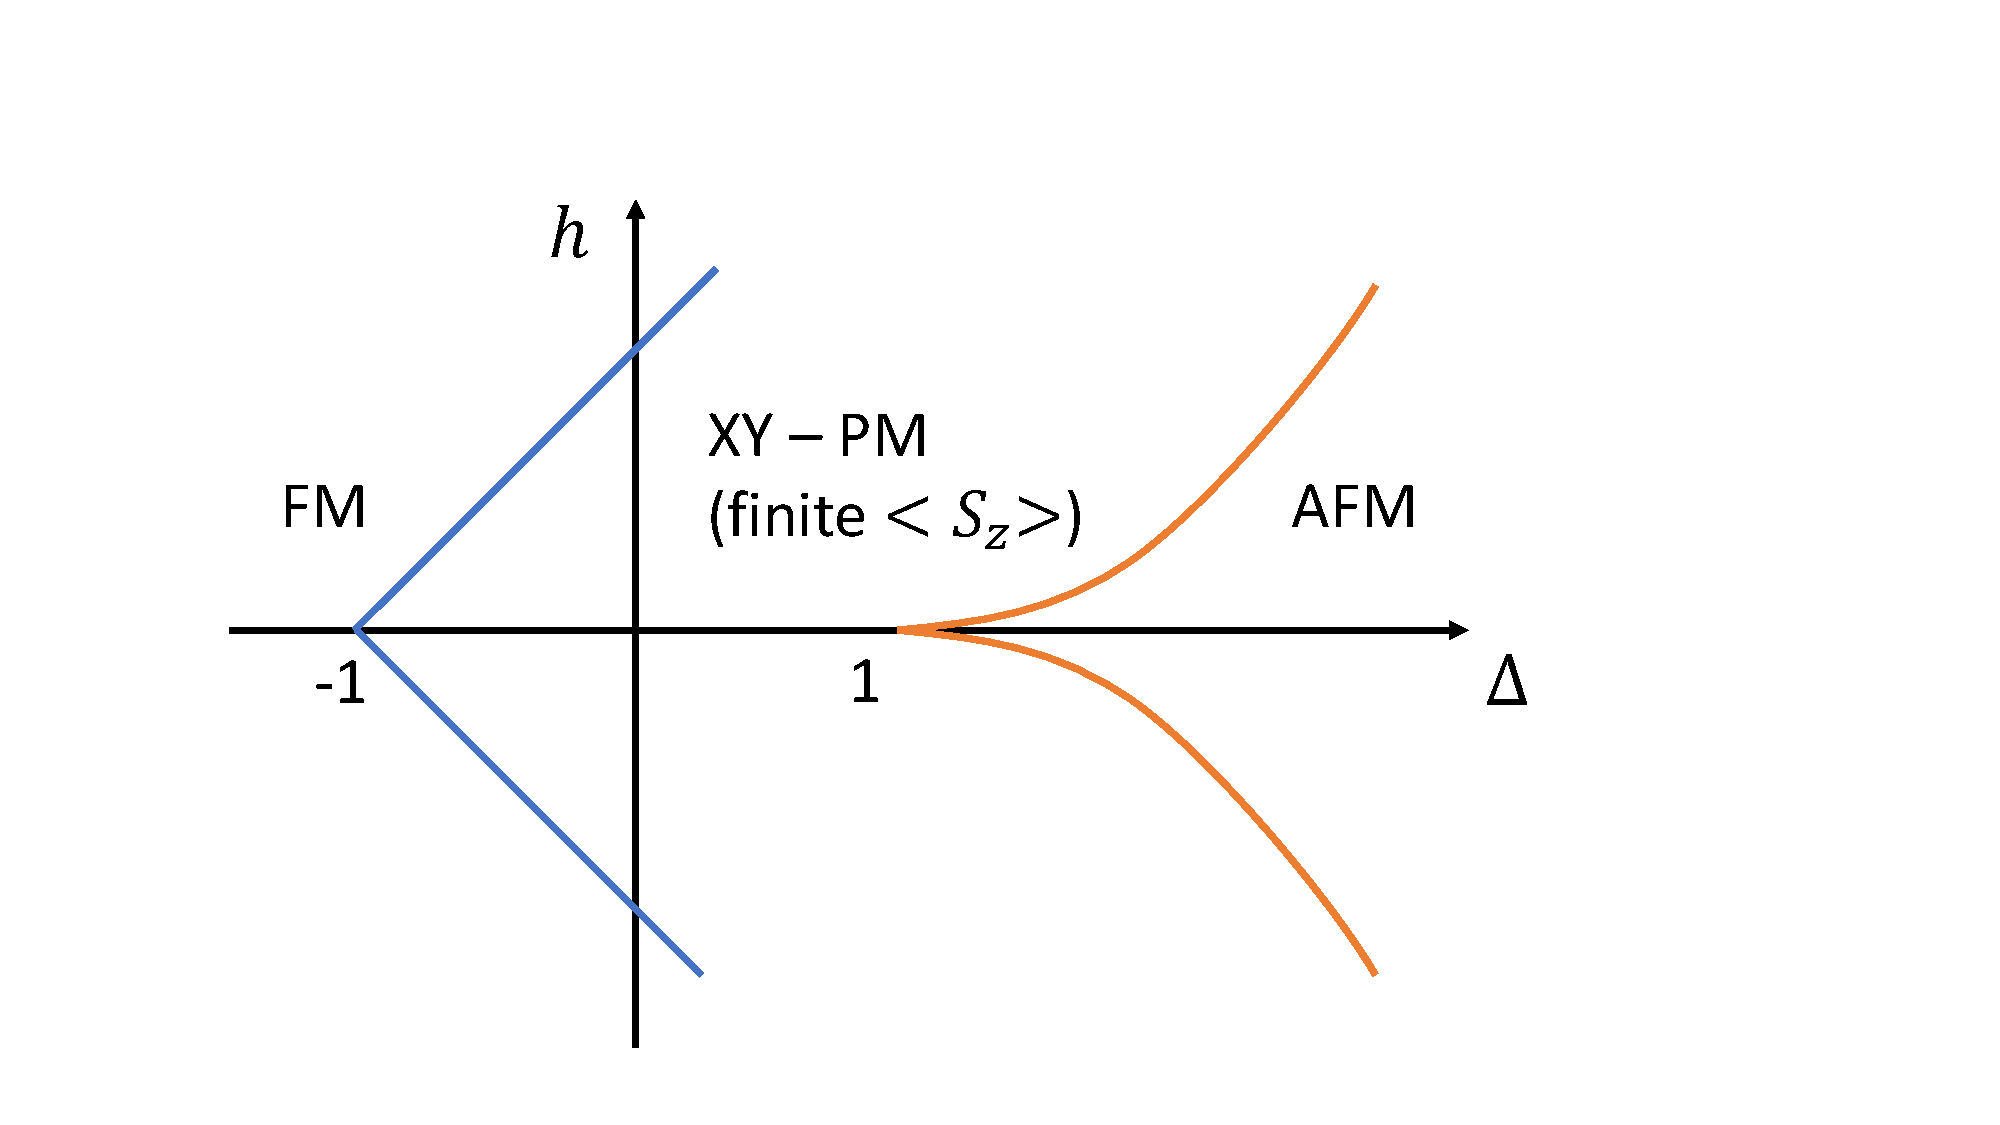
\includegraphics[width=\linewidth]{figs/CSC/phase_diagrams_Heisenberg.pdf}
    \vspace{0.5cm}
    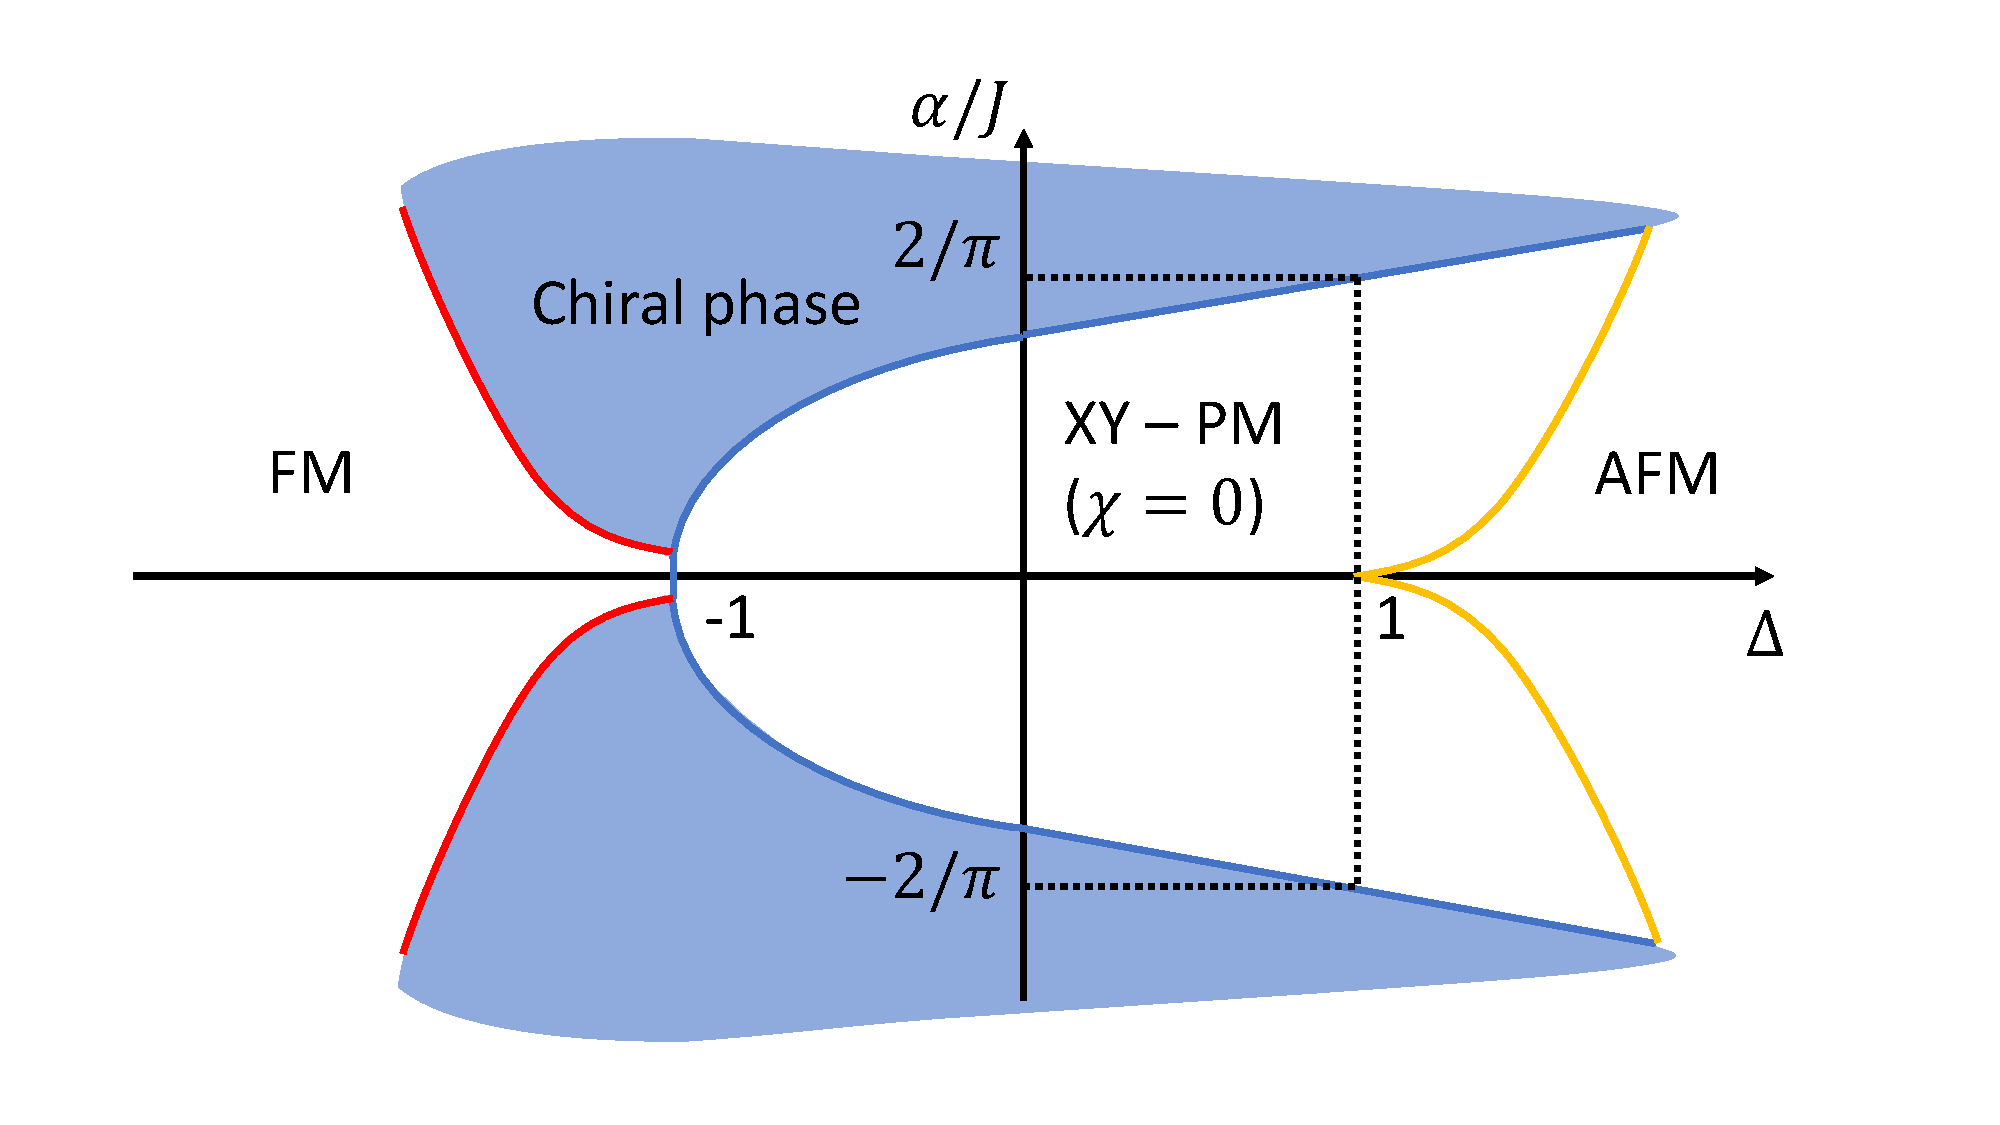
\includegraphics[width=\linewidth]{figs/CSC/phase_diagrams_chiral.pdf}
    \end{minipage}
\end{column}
\end{columns}
\end{frame}